\documentclass[10pt,compress]{beamer}
\usepackage{amsmath}
\usepackage{url}
\usepackage{ucs}
\usepackage[utf8x]{inputenc}
\usepackage[ngerman]{babel}
\usepackage{ulem}
\usepackage{multicol}
\usepackage{comment}
\usepackage{setspace}
\usepackage{color}

\title{Bloch-Gleichungen}
\date{10. Mai 2012}

\usetheme{Warsaw}
\usecolortheme{seahorse}
\usefonttheme{serif}
\useinnertheme{rectangles}
\usepackage{bookman}
\setbeamercovered{transparent}

\newcommand{\mb}{\mu_\mathrm{B}} 

\begin{document}
\frame[t] {
  \vfill
  \begin{center}
  \Huge Bloch-Gleichungen
  \end{center}
  \vfill
}

\section{Einleitung}
\subsection{Begriffe}
\frame {
  \frametitle{Übersicht}

  \begin{block}{ESR, NMR}
    Resonante {\color{red} Absorption} von {\color{red}Mikrowellenstrahlen} durch paramagnetische Ionen,
    Moleküle o.ä. in einem {\color{red}statischen Magnetfeld}.
  \end{block}

  \vfill

  \begin{block}{Bloch-Gleichungen}
    {\color{red} Bewegungsgleichungen} für die {\color{red} Magnetisierung $\vec M$} einer Probe unter dem Einfluss äußerer Magnetfelder.
  \end{block}
}

\subsection{Gleichungen}
\frame {
  \frametitle{Übersicht (2)}

  \begin{itemize}
  \item Magnetisches Moment 
  \begin{equation}
  \vec \mu = - \mb \left(\vec L + g_\mathrm{e} \vec S\right) = -g \mb \vec J = -\gamma \hbar \vec J
  \end{equation}
  \item Landé-Faktor (LS-Kopplung)
  \begin{equation}
  g=1+\frac{J(J+1)+S(S+1)-L(L+1)}{2J(J+1)}
  \end{equation}

  \item Hamilton-Operator 
  \begin{equation}
  \mathcal{H} = -\vec\mu \cdot \vec H = g \mb \vec H \cdot \vec J = g\mb H J_z
  \end{equation}
  mit den Eigenwerten 
  \begin{equation}
  E=g\mb Hm \text{\ \ \ \ \ \ \ \ }(m=-J,-J+1,\dots,J-1,J)
  \end{equation}

  \end{itemize}
}

\subsection{Zeeman-Aufspaltung}
\frame {
  \frametitle{Zeeman-Aufspaltung}

  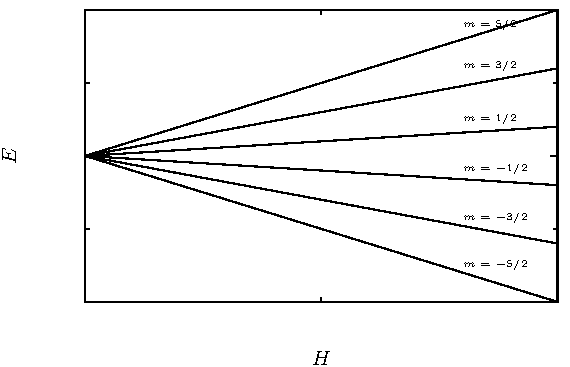
\includegraphics[scale=1.2]{zeeman.pdf}
}

\section{Bewegungsgleichungen}
\subsection{Herleitung}
\frame {
  \frametitle{Bewegungsgleichungen}
  \begin{itemize}
    \item Ausgangspunkt
    \begin{align}
    \label{H}
    \mathcal{H} &= -\vec \mu \cdot \vec H = \gamma \hbar \vec H \cdot \vec J = \gamma \hbar H J_z \\
    \label{mu}
    \vec \mu    &= - \gamma \hbar \vec J 
    \end{align}
    \item Erwartungswert des magnetischen Moments
    \begin{equation}
    \langle \vec \mu \rangle = \int \Psi^* \vec \mu \ \Psi \mathrm{d}\tau
    \end{equation}
    \item Heisenbergsche Bewegungsgleichung
    \begin{equation}
    \label{Heq}
    \frac{\mathrm{d}}{\mathrm{d}t} \langle \vec \mu \rangle = \frac{\mathrm{i}}{\hbar} \langle \left[\mathcal{H}, \vec \mu\right]\rangle
    \only<1> { + \langle \frac{\partial \vec \mu}{\partial t}\rangle }
    \only<3>{=-\mathrm{i}\gamma^2\hbar H \langle [ J_z, \vec J ]\rangle}
    \end{equation}
  \end{itemize}
}

\frame[t] {
  \frametitle{Bewegungsgleichungen (2)}

  \begin{itemize}
  \item Kommutatorrelation
  \begin{equation}
  \label{kommutator}
  [J_z, \vec J] = \mathrm{i} \left(J_y \vec e_x - J_x \vec e_y\right)
  \end{equation}


  \item Bewegungsgleichung
    \begin{align}
    \frac{\mathrm{d}}{\mathrm{d}t} \langle \vec \mu \rangle &= \frac{\mathrm{i}}{\hbar} \langle \left[\mathcal{H}, \vec \mu\right]\rangle
    \\ &=-\mathrm{i}\gamma^2\hbar H \langle [ J_z, \vec J ]\rangle
    \only<2->{\\ &\overset{(\ref{kommutator})}{=}\gamma^2 \hbar H \langle J_y \vec e_x - J_x \vec e_y \rangle}
    \only<3->{\\ &=\gamma \vec H \times \langle \vec \mu \rangle}
    \end{align}
  \end{itemize}

  \only<4->{
  \begin{block}{Bewegungsgleichungen}
   $$\frac{\mathrm{d}}{\mathrm{d}t} \langle \vec \mu \rangle = \gamma \vec H \times \langle \vec \mu \rangle$$
  \end{block}
  }
}

\frame {
  \frametitle{Bewegungsgleichungen (3)}

  Voraussetzungen:
  \begin{itemize}
  \item Dipole wechselwirken nicht miteinander
  \item isotropes System
  \item Gültigkeit der LS-Kopplung
  \end{itemize}

  \vfill
  \pause

  Magnetisierung:
  \begin{itemize}
  \item Magnetisierung
  \begin{equation}
  \vec M  = N \langle \vec \mu \rangle _\text{avg}
  \end{equation}
  \item Bewegungsgleichung für Magnetisierung
  \begin{equation}
  \frac{\mathrm{d}}{\mathrm{d}t} \vec M = \gamma \vec H \times \vec M
  \end{equation}
  \end{itemize}
}

\subsection{Lösungen}
\frame {
  \frametitle{Lösung im statischen Magnetfeld}

  \begin{itemize}
  \item statisches, zeitunabhängiges Magnetfeld $\vec H = H\vec e_z$
  \item Bewegungsgleichungen
  \begin{align}
  \dot \mu_x &= -\gamma H \mu_y \\
  \dot \mu_y &= \gamma H \mu_x \\
  \dot \mu_z &= 0
  \end{align}

  \pause

  \item DGl des harmonischen Oszillators
  \begin{equation}
  \ddot \mu_x = -(\gamma H)^2 \mu_x = -\omega^2 \mu_x
  \end{equation}

  \item Lösung
  \begin{align}
  \mu_x(t) &= \mu_x(0)\cos{\omega t} - \mu_y(0)\sin{\omega t} \\
  \mu_y(t) &= \mu_x(0)\sin{\omega t} + \mu_y(0)\cos{\omega t} \\
  \mu_z(t) &= \mu_z(0)
  \end{align}

  \item Lamorfrequenz: $f=\frac{\gamma H}{2\pi}$
  \end{itemize}
}

\frame {
  \frametitle{Lösung im statischen Magnetfeld (2)}

  \begin{center}
  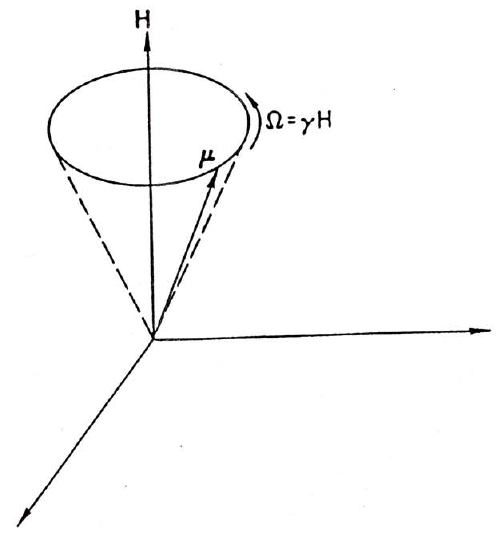
\includegraphics[scale=0.4]{fig22.png}

  Vektor $\vec \mu$ rotiert bei konstanter Länge und mit konstantem Winkel um das Magnetfeld $\vec H$
  \end{center}
}

\frame {
  \frametitle{Lösung im rotierenden Magnetfeld}

  \begin{itemize}
  \item Magnetfeld $\vec H = \vec H_1 + H_0 \vec e_z$
  \item Magnetfeld $H_1$
  \begin{equation}
  \begin{aligned}
    \vec H_1 &= 2 H_1 \cos{\omega t} \ \vec e_x =\\
             &= \underbrace{H_1\left(\vec e_x \cos{\omega t} + \vec e_y \sin{\omega t}\right)}_\text{1. Term} + \underbrace{H_1 \left(\vec e_x \cos{\omega t} - \vec e_y \sin{\omega t}\right)}_\text{2. Term}
  \end{aligned}
  \end{equation}

  \item 1. Term: Magnetfeld, das um $\vec H_0$ rotiert in gleicher Richtung wie die Larmorpräzession
  \item 2. Term: Magnetfeld, das um $\vec H_0$ rotiert entgegen der Lamorpräzession
  \item falls $H_1 \ll H_0$: 2. Term vernachlässigbar
  \end{itemize}
}

\frame {
  \frametitle{Lösung im rotierenden Magnetfeld (2)}

  Magnetfeld:
  \begin{equation}
    \vec H = \vec e_x H_1 \cos{\omega t} + \vec e_y H_1 \sin{\omega t} + \vec e_z H_0
  \end{equation}

  \begin{center}
  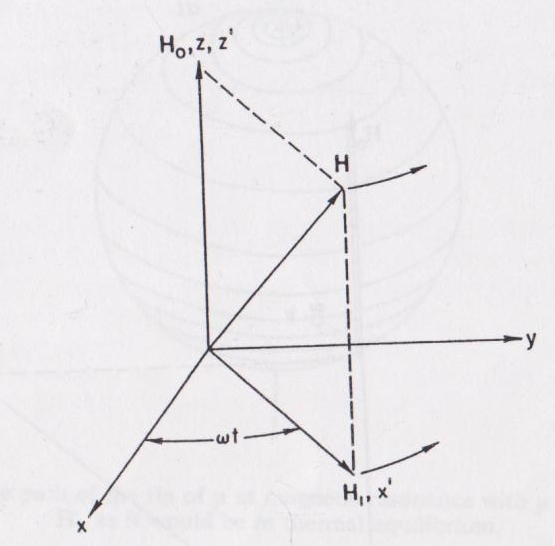
\includegraphics[scale=0.75]{fig23.jpg}
  \end{center}
}

\frame[t] {
  \frametitle{Lösung im rotierenden Magnetfeld (3)}

  Magnetfeld:
  \begin{equation}
    \vec H = \vec e_x H_1 \cos{\omega t} + \vec e_y H_1 \sin{\omega t} + \vec e_z H_0
  \end{equation}

  \begin{itemize}
    \item Transformation ins rotierende Bezugssystem
      \begin{equation}
      \frac{\mathrm{d}}{\mathrm{d}t} = \left(\frac{\mathrm{d}}{\mathrm{d}t}\right)_\text{rot} + \vec \omega \times
      \end{equation}
    \item hier:
    \begin{align}
    \only<2> { \phantom{\Rightarrow} \underbrace{\frac{\mathrm{d} \vec \mu}{\mathrm{d}t}}_{\gamma \vec H \times \vec\mu} &= \frac{\mathrm{d}\vec \mu'}{\mathrm{d}t} + \vec \omega \times \vec\mu \ \ \ \ \ \ \ \ \ \ \ \ \ \ \ \ \  }
    \only<3-> { \phantom{\Rightarrow} \frac{\mathrm{d} \vec \mu}{\mathrm{d}t} &= \frac{\mathrm{d}\vec \mu'}{\mathrm{d}t} + \vec \omega \times \vec\mu \ \ \ \ \ \ \ \ \ \ \ \ \ \ \ \ \  }
    \only<3-> { \\ \Rightarrow \frac{\mathrm{d} \vec \mu'}{\mathrm{d}t} &= \left(\gamma \vec H - \omega \vec e_z\right) \times \vec \mu}
    \end{align}
  \end{itemize}
}

\frame {
  \frametitle{Lösung im rotierenden Magnetfeld (4)}

  effektives Feld:
  \begin{equation}
  \vec H_e = \vec e_x' H_1 + \vec e_z' \left(H_0 - \frac{\omega}{\gamma}\right)
  \end{equation}

  \begin{center}
  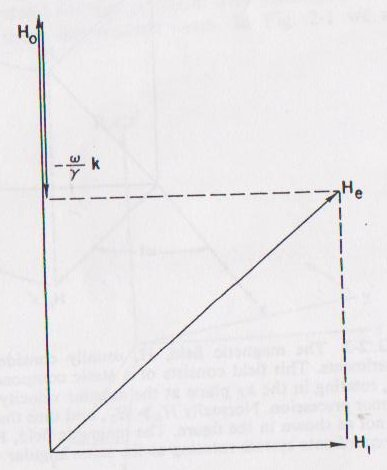
\includegraphics[scale=0.8]{fig24.jpg}
  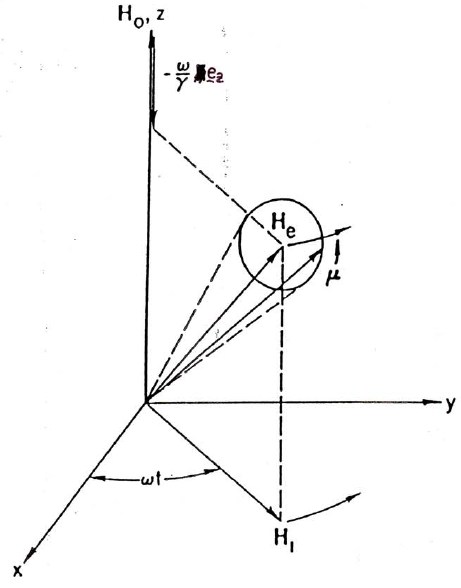
\includegraphics[scale=0.4]{fig25.png}
  \end{center}
}

\frame {
  \frametitle{Lösung im rotierenden Magnetfeld (5)}

  \begin{center}
  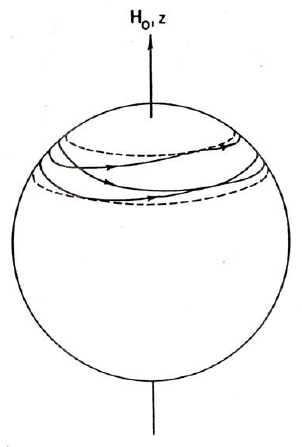
\includegraphics[scale=0.5]{fig26.png}

  Spitze des $\vec \mu$-Vektors abseits von Resonanz
  \end{center}
}

\frame {
  \frametitle{Lösung im rotierenden Magnetfeld (6)}

  \begin{center}
  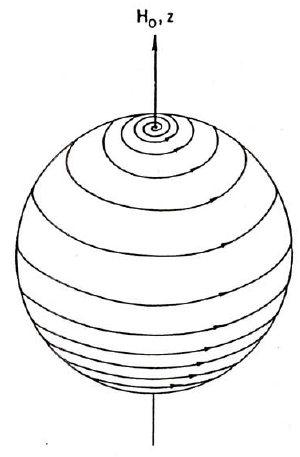
\includegraphics[scale=0.5]{fig27.png}

  Spitze des $\vec \mu$-Vektors bei Resonanz
  \end{center}
}

\frame {
  \frametitle{Lösung im rotierenden Magnetfeld (7)}

  \begin{center}
  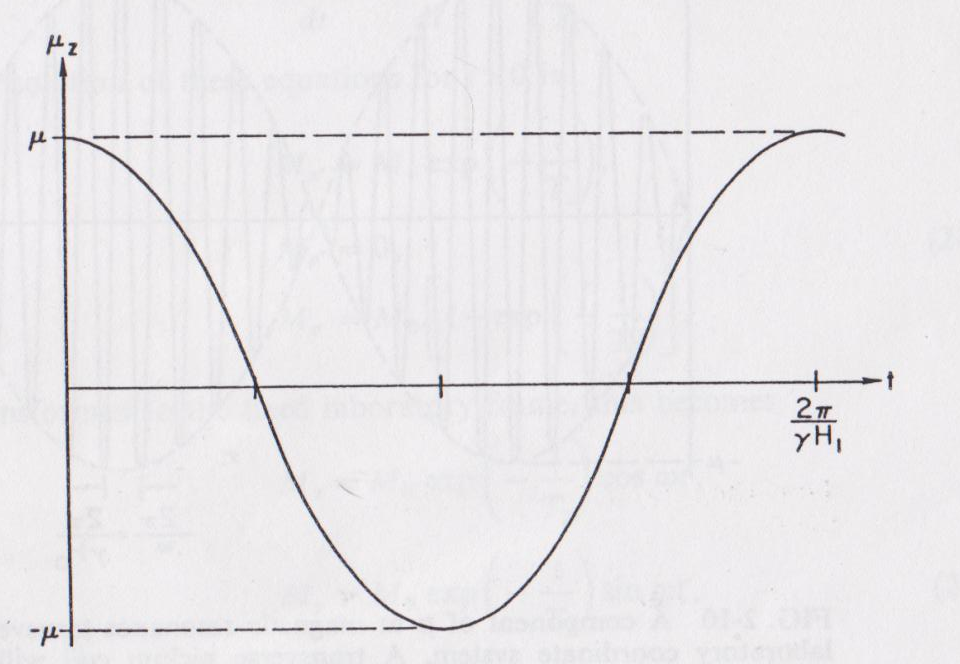
\includegraphics[scale=0.85]{fig28.png}

  Komponente von $\vec \mu$ entlang von $\vec H_0$ bei magnetischer Resonanz ($90^\mathrm{o}$-Puls)
  \end{center}
}

\section{Bloch-Gleichungen}
\subsection{Bloch-Gleichungen}
\frame {
  \frametitle{Bloch-Gleichungen}

  \begin{itemize}
  \item Relaxation statistisches Problem $\rightarrow$ Beschreibung durch Magnetisierung
  \item Annahme: lineare Antwort des Systems
  \end{itemize}

  \begin{align}
  \frac{\mathrm{d}M_x}{\mathrm{d}t} &= \gamma\left(\vec H \times \vec M\right)_x - \frac{M_x}{T_2} \\
  \frac{\mathrm{d}M_y}{\mathrm{d}t} &= \gamma\left(\vec H \times \vec M\right)_y - \frac{M_y}{T_2} \\
  \frac{\mathrm{d}M_z}{\mathrm{d}t} &= \gamma\left(\vec H \times \vec M\right)_z + \frac{M_0-M_z}{T_1}
  \end{align}

  \begin{itemize}
  \item $T_1$: longitudinale Relaxationszeit, Spin-Gitter-Relaxationszeit
  \item $T_2$: transversale Relaxationszeit, Spin-Spin-Relaxationszeit
  \end{itemize}
}

\subsection{Lösungen}
\frame {
  \frametitle{$90^\mathrm{o}$-Puls (NMR)}

  \begin{itemize}
  \item Magnetisierung wird gegenüber $\vec H_0$ um $90^\mathrm{o}$ ausgelenkt: $\vec M(t=0) = M_0 \vec e_x$
  \item Bloch-Gleichungen im rotierenden Bezugssystem
  \begin{align}
  \frac{\mathrm{d'}M_{x'}}{\mathrm{d}t} &=  - \frac{M_{x'}}{T_2} \\
  \frac{\mathrm{d'}M_{y'}}{\mathrm{d}t} &=  - \frac{M_{y'}}{T_2} \\
  \frac{\mathrm{d'}M_{z'}}{\mathrm{d}t} &=  \frac{M_0-M_{z'}}{T_1}
  \end{align}
  \only <1>
  {
  \item Lösungen (im rotierenden Bezugssystem; $\omega = \gamma H_0$)
  \begin{align}
  M_{x'} &= M_0 \exp{\left(-t/T_2\right)} \\
  M_{y'} &= 0 \\
  M_{z'} &= M_0 \left(1-\exp{\left(-t/T_1\right)}\right)
  \end{align}
  }
  \only <2>
  {
  \item Lösungen (im Laborsystem)
  \begin{align}
  M_{x} &= M_0 \exp{\left(-t/T_2\right)} \cos{\omega t}\\
  M_{y} &= M_0 \exp{\left(-t/T_2\right)} \sin{\omega t}\\
  M_{z} &= M_0 \left(1-\exp{\left(-t/T_1\right)}\right)
  \end{align}
  }
  \end{itemize}
}

\frame {
  \frametitle{$90^\mathrm{o}$-Puls (NMR) (2)}

  \begin{center}
  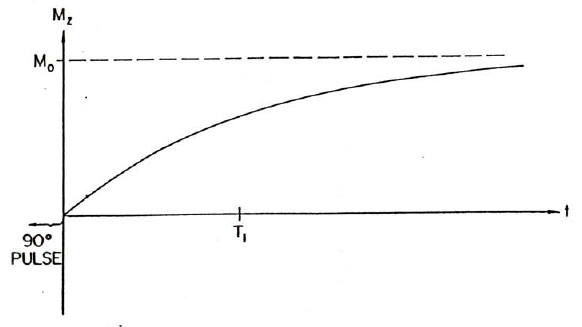
\includegraphics[scale=0.6]{fig211.png}

  Magnetisierung $\vec M$ entlang von $\vec H_0$ nach einem $90^\mathrm{o}$-Puls
  \end{center}
}

\frame {
  \frametitle{$90^\mathrm{o}$-Puls (NMR) (3)}

  \begin{center}
  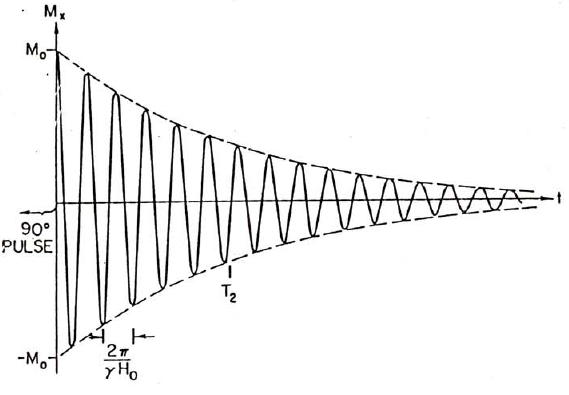
\includegraphics[scale=0.6]{fig212.png}

  Komponente von $\vec M$ transversal zu $\vec H_0$ nach einem $90^\mathrm{o}$-Puls
  \end{center}
}

\frame {
  \frametitle{Slow Passage (ESR)}
  
  \begin{itemize}
  \item $\vec H_0$ bzw. $\omega$ werden langsam gegenüber $T_1$, $T_2$ variiert
  \item effektives Magnetfeld
  \begin{equation}
  \vec H_e = \vec e_{x'} H_1 + \vec e_{z'} \left(H_0 - \frac{\omega}{\gamma}\right)
  \end{equation}
  \item Bloch-Gleichungen im rotierenden Bezugssystem
  \only<1>
  {
  \begin{align}
  \frac{\mathrm{d'}M_{x'}}{\mathrm{d}t} &=  \gamma \left(\vec H_e \times \vec M\right)_{x'} - \frac{M_{x'}}{T_2} \\
  \frac{\mathrm{d'}M_{y'}}{\mathrm{d}t} &=  \gamma \left(\vec H_e \times \vec M\right)_{y'} - \gamma H_1 M_{z'} - \frac{M_{y'}}{T_2} \\
  \frac{\mathrm{d'}M_{z'}}{\mathrm{d}t} &=  \gamma \left(\vec H_e \times \vec M\right)_{z'} + \frac{M_0-M_{z'}}{T_1}
  \end{align}
  }
  \only<2>
  {
  \begin{align}
  \frac{\mathrm{d'}M_{x'}}{\mathrm{d}t} &=  -\left(\gamma H_0 - \omega\right)M_{y'} - \frac{M_{x'}}{T_2} \\
  \frac{\mathrm{d'}M_{y'}}{\mathrm{d}t} &=  \left(\gamma H_0 - \omega\right)M_{x'} - \gamma H_1 M_{z'} - \frac{M_{y'}}{T_2} \\
  \frac{\mathrm{d'}M_{z'}}{\mathrm{d}t} &=  \gamma H_1 M_{y'} + \frac{M_0-M_{z'}}{T_1}
  \end{align}
  }
  \end{itemize}
}

\frame {
  \frametitle{Slow Passage (ESR) (2)}

  \begin{itemize}
  \item langsame Änderungen $\Rightarrow$ stationäre Lösung
  \begin{equation}
  \frac{\mathrm{d'}}{\mathrm{d}t} M_{x'} = \frac{\mathrm{d'}}{\mathrm{d}t} M_{y'} = \frac{\mathrm{d'}}{\mathrm{d}t} M_{z'} = 0
  \end{equation}
  \item Lösungen des linearen Gleichungssystems
  \begin{align}
  M_{x'} &= \frac{\gamma H_1 (\gamma H_0 - \omega) T_2^2}{1+(\gamma H_0 - \omega)^2 T_2^2 + \gamma^2 H_1^2 T_1 T_2}M_0 \\
  M_{y'} &= \frac{-\gamma H_1 T_2}{1+(\gamma H_0 - \omega)^2 T_2^2 + \gamma^2 H_1^2 T_1 T_2}M_0 \\
  M_{z'} &= \frac{1+(\gamma H_0 -\omega)^2 T_2^2}{1+(\gamma H_0 - \omega)^2 T_2^2 + \gamma^2 H_1^2 T_1 T_2}M_0
  \end{align}
  \end{itemize}
}

\frame {
  \frametitle{Slow Passage (ESR) (3)}

  \begin{itemize}
  \item komplexe Suszeptibilität $\chi=\chi'-\mathrm{i}\chi''$
  \item Dispersion
  \begin{equation}
  \chi' = \frac{M_{x'}}{H_1} = \frac{\gamma (\gamma H_0 - \omega) T_2^2 M_0}{1+(\gamma H_0 - \omega)^2 T_2^2 + \gamma^2 H_1^2 T_1 T_2}
  \end{equation}
  \item Absorption
  \begin{equation}
  \chi'' = \frac{-M_{y'}}{H_1} = \frac{\gamma T_2 M_0}{1+(\gamma H_0 - \omega)^2 T_2^2 + \gamma^2 H_1^2 T_1 T_2}
  \end{equation}

  \item Absorption: Lorentz-Kurve
  \end{itemize}
}

\frame {
  \frametitle{Slow Passage (ESR) (4)}

  \begin{center}
  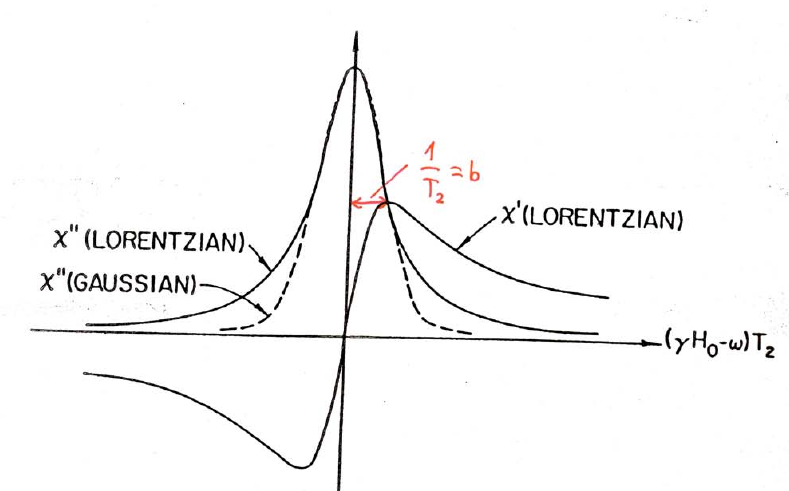
\includegraphics[scale=0.5]{fig220.png}
  \end{center}
}

\frame {
  \frametitle{ESR - Versuchsdurchführung}

  \begin{center}
  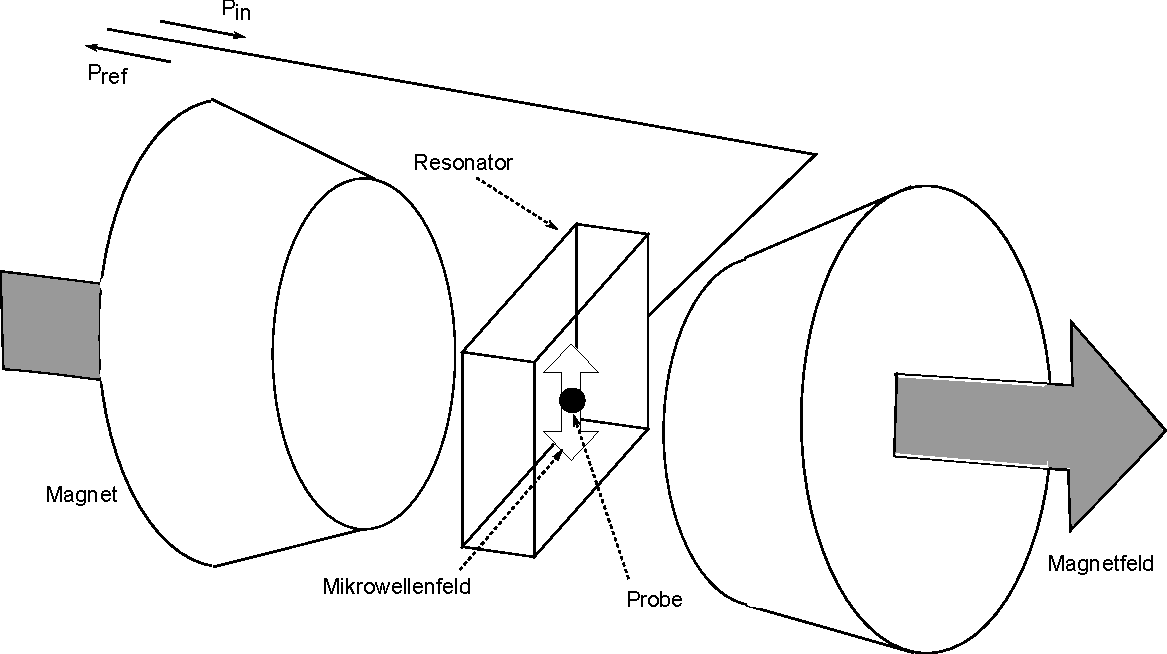
\includegraphics[scale=0.55]{Resonator.pdf}
  \end{center}
}

\frame {
  \frametitle{Quellen}

  \begin{center}
  {\huge Vielen Dank!}
  \end{center}

  \vfill

  Quellen:
  \begin{itemize}
    \item The Physical Principles of Electron Paramagnetic Resonance; Pake, Estle; 1973
    \item Einführung in die Festkörperphysik, Kittel
  \end{itemize}
}

\end{document}
